\documentclass[12pt]{article}
%%%%%%%%%%%%%%%%%%%%%%%%%%%%%%%%%%%%%%%%%

\usepackage{amscd}
\usepackage{amsmath}
\usepackage{amssymb}
\usepackage{amsthm}

\usepackage{subcaption}
\usepackage{hyperref}
\usepackage{paralist}
\usepackage{epsfig}
\usepackage{verbatim}
\usepackage{graphicx}
\usepackage{amsthm}
\usepackage{color}
%\usepackage[all,dvips]{xy}


\setlength{\textheight}{8.5in} \setlength{\topmargin}{0.0in}
\setlength{\headheight}{0.0in} \setlength{\headsep}{0.0in}
\setlength{\leftmargin}{0.5in}
\setlength{\oddsidemargin}{0.0in}
%\setlength{\parindent}{1pc}
\setlength{\textwidth}{6.5in}
%\linespread{1.6}

\newtheorem{definition}{Definition}
\newtheorem{problem}{Problem}

\newtheorem{theorem}{Theorem}[section]
\newtheorem{lemma}[theorem]{Lemma}
\newtheorem{note}[theorem]{Note}
\newtheorem{corollary}[theorem]{Corollary}
\newtheorem{prop}[theorem]{Proposition}

\newenvironment{nscenter}
 {\parskip=0pt\par\nopagebreak\centering}
 {\par\noindent\ignorespacesafterend}

%%%%%%%%%%%%%%%%%%%%%%%%%%%%%%%%%%%%%%%%%

\begin{document}
\thispagestyle{empty}

\bigskip
\bigskip

\begin{nscenter}
\textbf{\Large{A Comparison of Classifications in Handwritten Digit Recognition -- 50 \% Report}}
\end{nscenter}

\bigskip

\begin{nscenter}
{Siyang Xue and Tiancheng Liu}
\end{nscenter}

%This is where you would explain, in detail, what you plan to work on. This should be 1 to 3 pages in length. Here is an example of how you would cite your references in the body of your proposal.

\section{Problem Description}
\label{sec:problem}


Digit recognition has been a wide-spread and high-impact pattern recognition task, due to its simplicity: the background and the foreground (digits) are often well-separated, and the classes (categories) are limited to 10 (10 digits). Many researchers have benchmarked different methods on those datasets. Y. LeCun et al.\cite{lecun1998gradient} extracted their Mixed National Institute of Standards and Technology (MNIST) dataset from the National Institute of Standards and Technology (NIST) dataset, and made it normalized and available on their webpage\footnote{\url{http://yann.lecun.com/exdb/mnist/}}; they also provided early works on different classifications configurations in 1995, where linear classifiers, $k$-NN classifiers, and multiple variations of neural networks are investigated; a more complicated and complete comparisons can be found on the same webpage. A more recent work by CL Liu et al.\cite{liu2003handwritten} benchmarked methods of wider range on multiple datasets, on both feature extraction methods and classification methods.

What we are proposed is to further and more deeply investigate aspects of the digit recognition task. What we care about is how the different options in the classification pipeline affect the performance:
\begin{inparaenum} [\itshape a\upshape)]
\item How different normalization techniques influence the data quality, and how to provide a measurement (or at least, an intuition) on that;
\item how SIFT \cite{lowe2004distinctive}, HOG \cite{dalal2005histograms} and other feature extraction methods perform on feature extraction/generation; 
\item what is the suitable dimension reduction method for the task;
\item how the classifiers and the parameter setting affect the performance of the task.
\end{inparaenum} 

While the similar 


\section{Data Description}
\label{sec:data}
The data we used are from 2 different digit dataset, which are both well-known and widely-used for digit recognition:\begin{enumerate}[\itshape a\upshape)]
\item MNIST data\cite{lecun1998gradient}, which is the most-popular dataset for the task, all data are normalized beforehand;
\item USPS handwritten digits data\cite{hull1994database}, where the data was not normalized, and the testing data is harder than the training data.
\end{enumerate}

Some important information of the datasets are listed as follows:
\begin{enumerate}[\itshape a\upshape)]
\item MNIST: Total training set of 60,000 images; test set of 10,000 images; all the digits are normalized to size $20 \times 20$ and put in the middle of a $28 \times 28$ image.
\item USPS: 7291 for training and 2007 for testing; each image has 300 pixels ($10 \times 30$).
\end{enumerate}

In this report, we only work on a subset of MNIST dataset, where 6000 digits as training sample, and another 1000 digits as testing data.

All the training and testing samples are drawn respectively from the original training set and testing set. For training, we drawn 600 digits from each subject (0-9) randomly; 100 digits are drawn from each subject from the testing set to gather the subset of testing samples.

\begin{figure}[tbp]
	\centering
	\begin{subfigure}{.45\textwidth}
		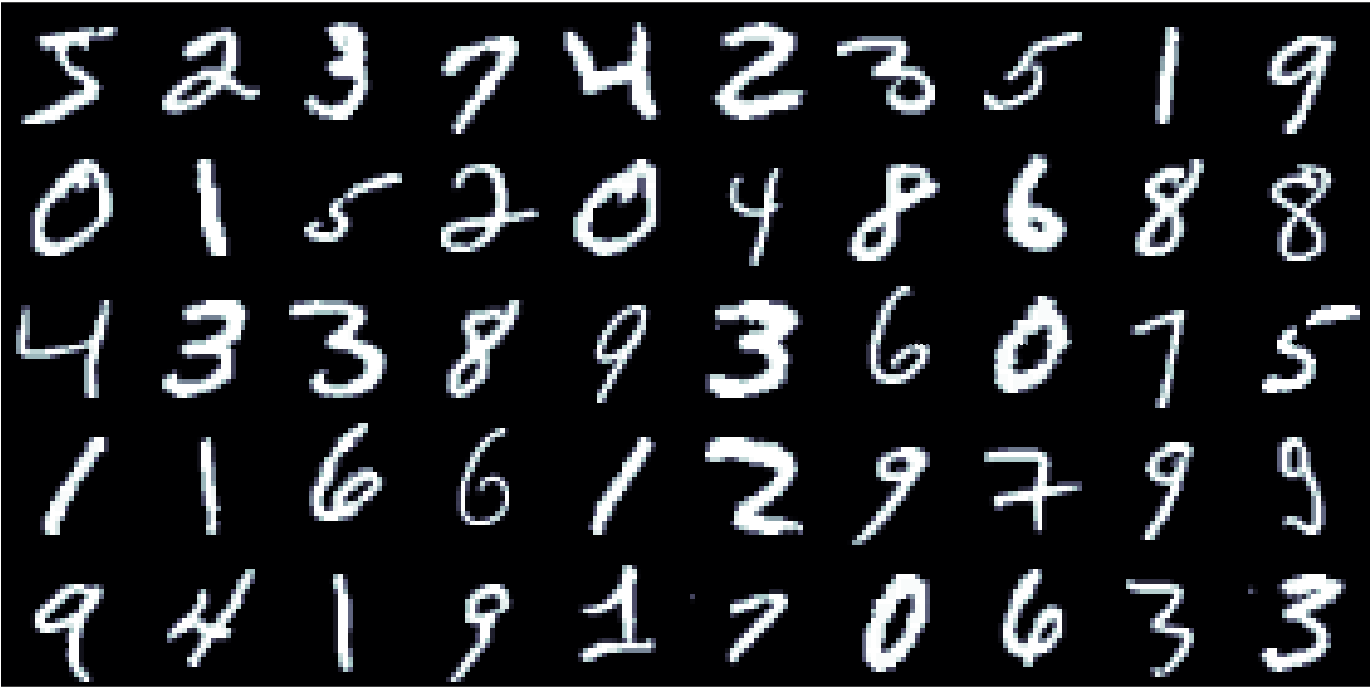
\includegraphics[height = 1.3in]{MNIST}		
		\caption{ }
	\end{subfigure}
	\begin{subfigure}{.45\textwidth}
		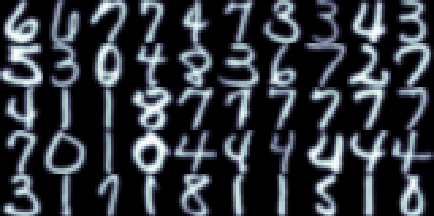
\includegraphics[height = 1.3in]{USPS}		
		\caption{ }
	\end{subfigure}
	\caption{Datasets: (a)~MNIST (b)~USPS}
\end{figure}

\section{Methods}
\label{sec:methods}

\subsection{Preprocessing}

The preprocessing step includes 3 sub-steps: normalization, feature extraction/generation, and dimension reduction. 

\subsubsection{Normalization}
The normalization process removes the size variation and illumination variation of the digits. For the MNIST dataset, as suggested by \cite{lecun1998gradient}, we removed the padding area to shrink each image from $28 \times 28$ to $20 \times 20$, which made the matching distance metric more precise and reduced the computational cost of further analysis. All the intensity data are normalized by the maximum intensity in the image, which removes the illumination variance between different images of digits. The result of the normalization can be seen in Figure \ref{fig:norm}.

\begin{figure}[tbp]
	\centering
	\begin{subfigure}{.45\textwidth}
		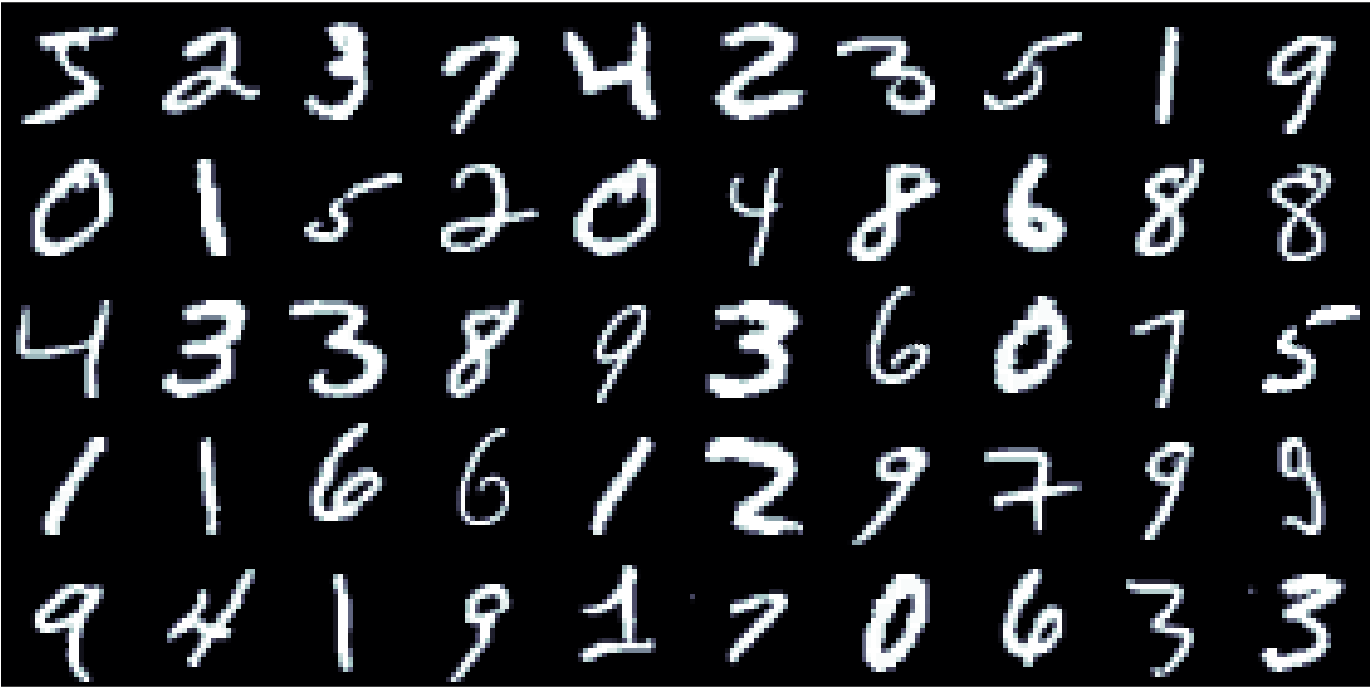
\includegraphics[height = 1.3in]{MNIST}		
		\caption{ }
	\end{subfigure}
	\begin{subfigure}{.45\textwidth}
		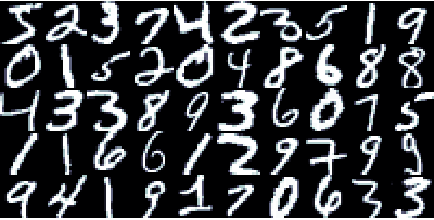
\includegraphics[height = 1.3in]{MNIST_norm}		
		\caption{ }
	\end{subfigure}
	\caption{Normalization of the dataset: (a)~MNIST(original) (b)~MNIST(normalized)}
	\label{fig:norm}
\end{figure}

\subsubsection{Feature Extraction}
Feature extraction/generation methods based on gradient and local invariant feature detectors are investigated. To be specific, in this report, we investigated two common feature extraction strategy in the Computer Vision society: a) HOG features and b) Scale-invariant feature transform (SIFT) features.

\subsubsection*{HOG Features}
 Histograms of Oriented Gradients(HOG)\cite{dalal2005histograms}\cite{felzenszwalb2010object} is a feature selection method based on detection of local gradient distributions. Not only detection of edge positions, but also intensity normalization is included in this method, making it invariant to the shadows or illumination difference of the sample image. A lot of HOG implements are proposed, with different parameter and slightly differently designed histogram calculating schemes. In this project, we will focus mainly on a Felzenszwalb et al. version\cite{felzenszwalb2010object}  of HOG, for its relatively fewer features in selecting, as we only care about the distinguish from 0 to 9 in handwritten digits recognition, and too many features could be disturbing.

First, in order to identify the local edges orientation and intensity, the image is divided into cells of $4\time4$. In each cell, a histogram of the gradient orientation is created by dividing the orientations $\theta$ of the gradient evenly into 9 bins, and each vote has the weight of $r$(i.e. the magnitude of the coordinate pixel). Therefore, for a $ w\times h$ image,  a $w/4 \times h/4 \times 9$ cell feature map $C$ is created. 

Then, for each items of the feature map $C(i,j,:)$, it is normalized with its 8-neighbor items by creating a $4\times 9$ matrix.
\begin{equation}
\begin{aligned}
HOG(i,j,:,:) =&  \left[\begin{array}{c}
C(i,j,:)./N_{-1,-1}(i,j,:)\\
C(i,j,:)./N_{-1,+1}(i,j,:)\\
C(i,j,:)./N_{+1,+1}(i,j,:)\\
C(i,j,:)./N_{+1,-1}(i,j,:)\end{array}\right]\\
 N_{\delta,\gamma} =&\\
 & (||C(i,j,:)||^2+||C(i+\delta,j,:)||^2+||C(i,j+\gamma,:)||^2+||C(i+\delta,j+\gamma,:)||^2)^{\frac{1}{2}}
\end{aligned}
\end{equation}\cite{felzenszwalb2010object}
Each matrix is then reshaped into a 36 dimensional vector, resulting a overall $ w/4 \times h/4 \times 36$ feature map.

Finally, the now normalized feature map is compressed to 31 features per cell, using PCA projecting the features to 31 most variant dimensions in the $ w/4 \times h/4 $ features of the image. This step is different from the later dimension-reduction step of all the images in the training set in that it calculates the principal components within the same image and is aimed at eliminating the specific minor noises of a particular image.
\begin{figure}[h]
\centering
	\begin{subfigure}{.85\textwidth}
		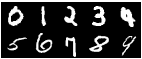
\includegraphics[height = 2.1in]{image.png}		
		\caption{ }
	\end{subfigure}
	\begin{subfigure}{.85\textwidth}
		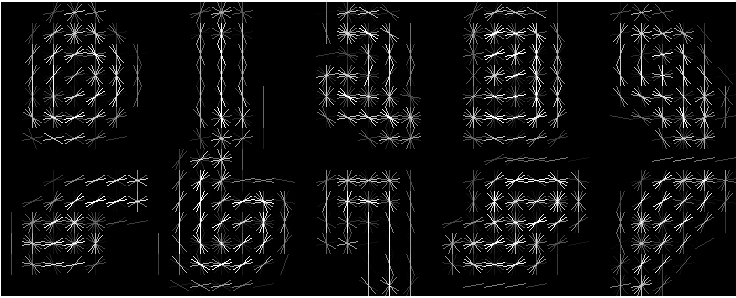
\includegraphics[height = 2in]{hog.png}	
		\caption{ }
	\end{subfigure}
	\caption{ (a)handwritten digits 0-9 from MNIST (b)HOG features of handwritten digits 0-9}
	\label{fig:norm}
	\end{figure}

The original images, and the HOG features of digits from 0 to 9 is shown in Figure 1 and Figure 2 respectively. As shown in the figures, the HOG features well describe the outlines of the digits. A digit written with a thinner line( such as the '9' in Figure 1) does not make much difference in the HOG feature description with digits written with thicker strokes, making the features resistant to the irrelevant factors.

\subsubsection*{SIFT Features}
 
Scale-invariant feature transform is a popular feature extraction technique introduced by David Lowe in his 2004 paper \cite{lowe2004distinctive}. The process consists of typically three steps: a) Detection of scale-space extrema, where image pyramid is generated using a set of different-scaled Gaussian kernels, and the extrema is detected in a spatial-hierarchical neighborhood; b) Accurate keypoint localization, where the extrema of low contrast and extrema near the image boundary are discarded; c) Orientation assignment, where each keypoint is assigned several orientations according to its spatial neighbors.

The SIFT features are often applied in object detection, face recognition, and other related tasks \cite{yilmaz2006object, dalal2005histograms}, due to its robustness against image scaling, image rotation, and certain kinds of noise. In these applications, the SIFT features (keypoints) are extracted, and oftentimes, it is followed by extracting the HOG features of the spatial neighborhood of the keypoints, to generate a feature descriptor \cite{lowe2004distinctive}.

However, this feature extraction strategy is ineffective for the MNIST dataset. In the experiment, we found all the images have only a few feature points to be extracted ($\leq 4$), which is insufficient to describe the image (see Figure \ref{fig:SIFT}); some image even failed on SIFT, that means it have no SIFT feature to extract. Furthermore, it may not be a desirable choice for digits dataset, where we have 6 and 9 with the same topology, and the rotation invariant property of SIFT would made it impossible to distinguish the above 2 digits. Therefore, in this report, we do not use SIFT as a feature extraction technique, and only HOG is used to generate feature descriptors.

\begin{figure}[tbp]
	\centering
	\begin{subfigure}{.45\textwidth}
		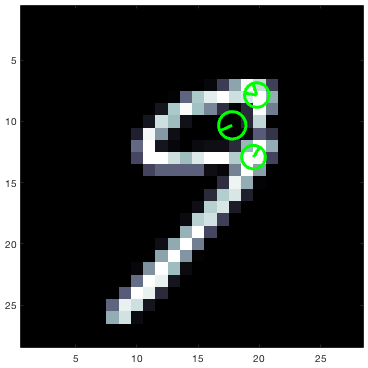
\includegraphics[height = 2.5in]{SIFT}		
		\caption{ }
	\end{subfigure}
	\begin{subfigure}{.45\textwidth}
		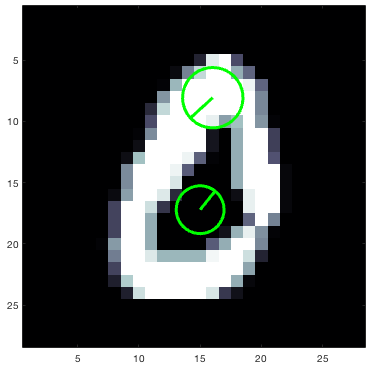
\includegraphics[height = 2.5in]{SIFT_2}		
		\caption{ }
	\end{subfigure}
	\caption{Handwritten digits with their SIFT features: (a)~A handwritten 9 (b)~ A handwritten 0}
	\label{fig:SIFT}
\end{figure}


However, for further study, if we are to investigate faces, SIFT would be a good choice for extracting the keypoints in a more complex context, and the the invariant properties of the SIFT would help the recognition.
 
 \subsubsection{Dimension Reductions}
 
The dimension reduction methods used in this report can be categorized into 2 groups: linear and nonlinear. For linear method, we apply the conventional PCA; both kernel method (Kernel-PCA) and manifold learning method (LLE) are investigated as nonlinear methods. Experiments are conducted to compare the effectiveness and efficiency of the methods.

 
\subsection{Clustering}
After the preprocessing, we plan to investigate clustering methods on the new feature space. The clustering methods such as k-means, EM and DBSCAN will be investigated to show the intrinsic nature of the dataset, and will be used as references to justify and validate the further classification process. This part is to be discussed in the future report.

\subsection{Classification}
Different classification methods are to be investigated in the final stage. In this report, we used $k$NN classifier for simplicity to appreciate the techniques introduced in the former sections.

\section{Results}
In this section, we discuss the differences of the performances of the classifier with input types: features without selection, HOG features selected with raw data, and further HOG features selected with normalized data over the several dimensional reduction methods. Running time and classification accuracy are both included in the measurement of the performance.
\begin{table}[h!]
\centering
\caption{Accuracy and Running Time Without Feature Selection or Normalization}
\label{tab:res}
\begin{tabular}{cccccc}
\hline
& \textbf{None} & \textbf{PCA} & \textbf{Poly} & \textbf{Gaussian} & \textbf{LLE} \\
 \hline
Accuracy(\%)               &   87.80     &   90.20 &90.10 &91.90 &91.90  \\
\hline
Running Time(s)    & --            &  5.72    &    76.68 & 80.20 &38.95\\
\hline
\end{tabular}
\end{table}
\begin{table}[h!]
\centering
\caption{Accuracy and Running Time With Normalization and Without Feature Selection}
\label{tab:res}
\begin{tabular}{cccccc}
\hline
& \textbf{None} & \textbf{PCA} & \textbf{Poly} & \textbf{Gaussian} & \textbf{LLE} \\
 \hline
Accuracy(\%)               &   93.00    &   93.30 &92.60 &94.00 &95.10  \\
\hline
Running Time(s)    & --            &  0.61    &    283.50 & 295.91 &18.71\\
\hline
\end{tabular}
\end{table}
\begin{table}[h!]
\centering
\caption{Accuracy and Running Time Without Normalization and With Feature Selection}
\label{tab:res}
\begin{tabular}{cccccc}
\hline
& \textbf{None} & \textbf{PCA} & \textbf{Poly} & \textbf{Gaussian} & \textbf{LLE} \\
 \hline
Accuracy(\%)               &   93.90     &   95.90 &95.20 &96.20 &96.50  \\
\hline
Running Time(s)    & 14.70       &  17.01    & 99.61 &107.39   & 101.39\\
\hline
\end{tabular}
\end{table}
\begin{table}[h!]
\centering
\caption{Accuracy and Running Time With Normalization and With Feature Selection}
\label{tab:res}
\begin{tabular}{cccccc}
\hline
& \textbf{None} & \textbf{PCA} & \textbf{Poly} & \textbf{Gaussian} & \textbf{LLE} \\
 \hline
Accuracy(\%)               &   95.40     &   95.70 &95.10 &95.90 &96.50  \\
\hline
Running Time(s)    & 7.24       &  7.98       & 92.52 &101.76 &45.01\\
\hline
\end{tabular}
\end{table}
\subsection{Comparison on Normalization}
Comparing Table 3 with Table 4, the accuracy of features with normalization previous to dimension reduction is not higher than that of features without normalization. That is partly because of the information loss in the gradient near the frame of the digits. On the contrary, normalization performed with no dimension reduction helps to improve the accuracy of the classification by eliminating irrelevant part of the features, as there is no dimension reduction process selecting the major features here.
At the same time, normalization will decrease the dimension of features, thus decreasing the running time of dimension reduction method.
\subsection{Comparison on Feature Selection}
By comparing Table 3 with Table 1, and Table 4 with Table 2, basically a increase of accuracy of 4\% to 7\% is achieved by selecting HOG features. Better edge detection and shadow invariant property of the HOG features might contribute to this increase. The increase is especially large in the case of none dimension reduction ( 7.6\% ) as the classification performance is more dependent to the feature quality with no further dimension reduction step.
The running time is longer with feature selection, as the original dimension of the data is 784, and the selected feature dimension here is 775, so there is no much decrease in the dimension reduction process, and the increase in computational complexity comes from the HOG feature detection step. This increase, however, is minor(less then 10 percent) compared to the accuracy improvement.
\section{Conclusion}
In this report, we investigated the normalization method, feature selection methods, and dimension reduction methods, with a simple $k$NN classifier. Several experimental comparisons are also made to appreciate the effect of each step. The conclusions are as follows: a) HOG feature are used for feature selection, and is helpful for digit recognition; b) SIFT is not suitable for digit recognition, due to the simple structure of the digit images, and the topology similarity too high between the digits can make it impossible to distinguish the digits from others; c) Dimension reduction methods help the recognition, and the nonlinearity of the dataset is demonstrated.

For next step, we would begin to consider clustering methods and different classification methods.
\bibliographystyle{plain}
\bibliography{references}


\newpage
\begin{nscenter}
\Large{Tiancheng's contribution}
\end{nscenter}
\begin{itemize}
\item Set up the Github repository for collaboration
\item Normalized the MNIST dataset (max-normalization \& depadding)
\item Investigated the SIFT, and analysis why it is not a desirable choice for digit recognition.
\item Conducted the experimental comparison of normalized v.s. original, based on Siyang's HOG feature extraction
\item Fixed the LLE code
\end{itemize}

\newpage
\begin{nscenter}
\Large{Siyang's contribution}
\end{nscenter}
\begin{itemize}
\item Investigated the HOG, and discussed how it improved the performance of classification by detecting edges more accurately
\item Running the experimental comparison between the feature selected and none feature selected classification.
\item Fixed the kernel-PCA code
\end{itemize}



%%%%%%%%%%%%%%%%%%%%%%%%%%%%%%%%%%%%%%%%%






\end{document} 
